\subsection*{Task 1.2}
\subsubsection*{Task 1.2.1}
The coordinate frame can be assumed to be unambiguous if it is defined in relation to a solid object. This means although the relative transformation is clear from the matrices, the actual position after the transformation depends on the initial frame A. Otherwise the transformation order should be clear from the notation. 
\subsubsection*{Task 1.2.2}
See figure \ref{fig:task_1_2_2}.
\begin{figure}[H]
	\centering
	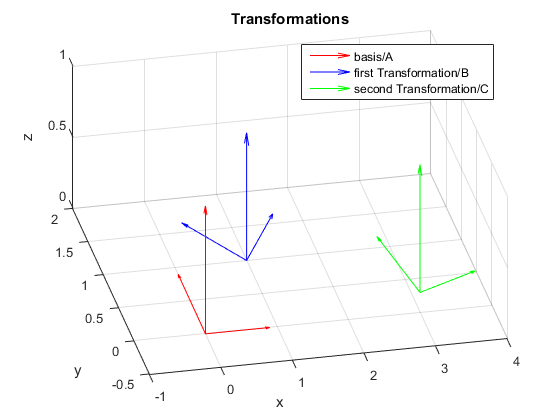
\includegraphics[width= \textwidth ]{CoordSys_2.png}
	\caption{The three frames A,B and C visualized}
	\label{fig:task_1_2_2}
\end{figure}